\documentclass{beamer}

\usepackage[utf8]{inputenc}
\usepackage{default}
\usepackage{xcolor}
\usepackage{tikz}
\usepackage{pgfplots}
\usepackage{pgfplotstable}
\usepackage{accents}
\usepackage[most]{tcolorbox}
\pgfplotsset{compat=1.5}
\usetikzlibrary{patterns,decorations.markings}

\definecolor{mygreen}{RGB}{0, 153, 0}

\usetheme{Berlin}
\setbeamertemplate{footline}{% 
  \hfill% 
  \usebeamercolor[fg]{page number in head/foot}% 
  \usebeamerfont{page number in head/foot}% 
  \insertframenumber%
  %\,/\,\inserttotalframenumber
  \kern1em\vskip2pt% 
}
% \setbeamertemplate{footline}[frame number]

\newcommand{\hvv}[1]{\accentset{\rightharpoonup}{#1}}
\newcommand{\grad}{\ensuremath{\hvv{\nabla}}}

\definecolor{contigColor}{RGB}{170, 255, 184}
\definecolor{distribColor}{RGB}{138, 180, 247}

\title{Parallel gyrokinetic simulations with Python}
\author{Emily Bourne\inst{1} \and Yaman G\"u\c{c}l\"u\inst{2}}
\institute{\inst{1}Technische Universit\"at M\"unchen, Germany \and \inst{2}Max-Planck-Institut f\"ur Plasmaphysik, Garching, Germany}
\date{25th October 2018}

\begin{document}
\begin{frame}
 \maketitle
\end{frame}

\begin{frame}{Motivation}
 Scientific Computing requirements:
 \begin{itemize}
  \item Fast algorithm prototyping
  \item Flexible
  \item Interactive
  \item Single-core optimization
  \item Shared-memory and MPI parallelization
  \item Strict quality control
 \end{itemize}

\end{frame}

\begin{frame}{Strategy}
 \begin{itemize}
  \item Code is written in Python
  \item Bottlenecks are translated automatically to Fortran using pyccel
 \end{itemize}
\end{frame}

\begin{frame}{Thanks}
 Thanks to Ahmed Ratnani and Sa\"id Hadjout for their work on pyccel.
\end{frame}


\begin{frame}{Outline}
 \setcounter{tocdepth}{1}
 \tableofcontents
\end{frame}

\section{Screw-Pinch Simulation}

\begin{frame}{Screw-Pinch Simulation\footnote{G. Latu, M. Mehrenberger, Y. Güçlü, M. Ottaviani, E. Sonnendrücker, “Field-aligned interpolation for semi-lagrangian gyrokinetic simulations” Journal of Scientific Computing, vol. 74, pp. 1601–1650, March 2018}}
\begin{minipage}{.45\textwidth}
 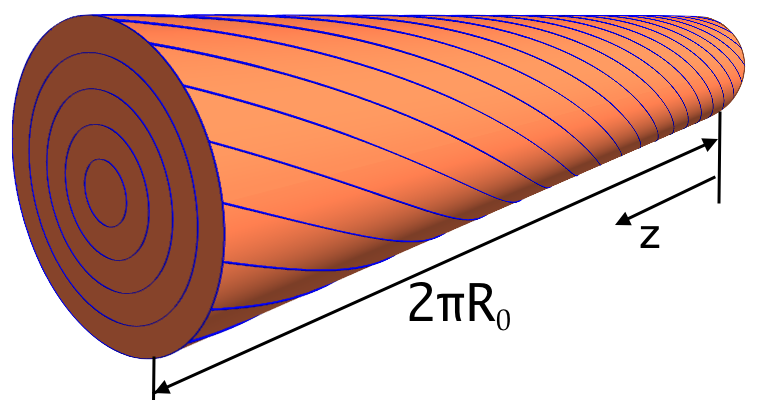
\includegraphics[width=\textwidth]{geometry_screw_pinch.png}
\end{minipage}
\begin{minipage}{.5\textwidth}
 \begin{equation*}
 \partial_t f + \{\phi,f\} + v_\parallel \grad_\parallel f - \grad_\parallel\phi\,  \partial_{v_\parallel} f=0
\end{equation*}
\begin{equation*}
 \{\phi,f\}=-\frac{\partial_\theta\phi}{rB_0}\partial_r f + \frac{\partial_r\phi}{rB_0}\partial_\theta f
\end{equation*}
\end{minipage}

\vspace{1em}
\begin{equation*}
 -\left[\partial_r^2\phi + \left(\frac{1}{r}+\frac{\partial_rn_0}{n_0}\right)\partial_r\phi+\frac{1}{r^2}\partial_\theta^2\phi\right]+\frac{1}{T_e}\phi = \frac{1}{n_0}\int_{-\infty}^{+\infty}(f-f_{eq})dv_\parallel
\end{equation*}
\end{frame}

\begin{frame}{Advection Operators}
\centering
\tcbox{$\partial_t f + \{\phi,f\} + v_\parallel \grad_\parallel f - \grad_\parallel\phi\,  \partial_{v_\parallel} f=0$}
\vspace{-2em}
\begin{equation*}
 \{\phi,f\}=-\frac{\partial_\theta\phi}{rB_0}\partial_r f + \frac{\partial_r\phi}{rB_0}\partial_\theta f
\end{equation*}

\begin{itemize}
\item Lie and Strang splitting are used for the predictor and corrector steps
\end{itemize}

\begin{minipage}[b]{.45\textwidth}
 Advection on poloidal plane:
 \vspace{.3em}
 
 Advection on flux surface:
 \vspace{.3em}
 
 V-parallel advection:
 \vspace{.4em}
\end{minipage}
\begin{minipage}[b]{.5\textwidth}
 \begin{align}
 \partial_t f + \,\,\,\,\,\,\,\,\,\,\,\,\, \{\phi, f\} &= 0 \label{Eq::Advection3}\\
 \partial_t f + \,\,\,\,\,\,\,\, v_\parallel \cdot \nabla_\parallel f &= 0 \label{Eq::Advection1}\\
 \partial_t f + \nabla_\parallel \phi\,\, \cdot \partial_{v_{\parallel}} f &= 0 \label{Eq::Advection2}
\end{align}
\end{minipage}

\end{frame}

\begin{frame}{Advection Operators}
\begin{minipage}[t]{.5\textwidth}
 \bf Advection on poloidal plane:
 \end{minipage}
 \hspace{.05\textwidth}
 \begin{minipage}[t]{.35\textwidth}
 $\partial_t f + \,\,\,\,\,\,\,\,\,\,\,\,\, \{\phi, f\} = 0$
\end{minipage}
 
 \begin{itemize}
   \item Semi-lagrangian method
   \item Explicit second order Euler determines trajectory
  \end{itemize}
  
\begin{minipage}[t]{.45\textwidth}
 \bf Advection on flux surface:
 \end{minipage}
 \hspace{.1\textwidth}
 \begin{minipage}[t]{.4\textwidth}
 $\partial_t f + \,\,\,\,\,\,\,\, v_\parallel \cdot \nabla_\parallel f = 0$
\end{minipage}
 
 \begin{itemize}
   \item Constant velocity semi-lagrangian method
  \end{itemize}
  
\begin{minipage}[t]{.45\textwidth}
 \bf V-parallel advection:
 \end{minipage}
 \hspace{.1\textwidth}
 \begin{minipage}[t]{.4\textwidth}
 $\partial_t f + \nabla_\parallel \phi\,\, \cdot \partial_{v_{\parallel}} f = 0$
\end{minipage}
 
 \begin{itemize}
   \item Constant velocity semi-lagrangian method
   \item $\nabla_\parallel \phi$ determined using 6th order finite differences
  \end{itemize}
  
\end{frame}

\begin{frame}{Advection on flux surface}
\begin{overlayarea}{\textwidth}{8cm}
\begin{equation}
 \partial_t f + v_\parallel \cdot \nabla_\parallel f = 0
\end{equation}

\only<1>{Magnetic Field lines:}
\only<2>{Retrace path:}
\only<3>{Find points either side for Lagrange interpolation:}
\only<4>{Use $\theta$-spline to find values:}
\begin{tikzpicture}[scale=0.8]
\only<1->{
  \node at (-1,2.5) {$r\cdot \theta$};
  \node at (5,-1) {$z$};
  \foreach \i in {0,2,...,10}
  {
   \foreach \j in {0,1,...,5}
   {
    \fill (\i,\j) circle (0.1);
   }
  }
   \foreach \j in {1,2,...,5}
   {
    \foreach \i in {2,4,...,10}
    {
     \draw[green] (\i,\j) -- (0,\j-\i*0.05);
    }
   }
  }
  \only<2->{
   \draw[red,thick] (10,5) -- (5,4.75);
   \fill[red] (5,4.75) circle (0.1);
   \node[below,red] at (7.5,4.9) {\footnotesize $-v_\parallel\cdot dt$};
  }
  \only<4->{
  \foreach \i in {0,2,...,10}
  {
    \draw (\i,0) -- (\i,5);
  }
  }
  \only<3->{
   \fill[blue] (2,4.6) circle (0.1);
   \fill[blue] (4,4.7) circle (0.1);
   \fill[blue] (6,4.8) circle (0.1);
   \fill[blue] (8,4.9) circle (0.1);
  }
\end{tikzpicture}
\end{overlayarea}

\end{frame}

\begin{frame}{Quasi-Neutrality Equation}
 \begin{equation*}
 -\left[\partial_r^2\phi + \left(\frac{1}{r}+\frac{\partial_rn_0}{n_0}\right)\partial_r\phi+\frac{1}{r^2}\partial_\theta^2\phi\right]+\frac{1}{T_e}\phi = \frac{1}{n_0}\int_{-\infty}^{+\infty}(f-f_{eq})dv_\parallel
\end{equation*}
\vspace{2em}

\begin{itemize}
 \item Theta component is handled using Fourier transforms
 \item Poisson equation solved using Finite Elements on a b-spline basis
\end{itemize}
\end{frame}

\begin{frame}{Screw-Pinch Simulation - Method summary}
\begin{enumerate}
 \item Compute $\phi$ from $f^n$ by solving the quasi-neutrality equation \label{get phi}
 \item Compute $f^{n+\frac{1}{2}}$ from $f^n$ using Lie splitting
 \item Compute $\phi$ from $f^{n+\frac{1}{2}}$ by solving the quasi-neutrality equation again
 \item Compute $f^{n+1}$ from $f^n$ using Strang splitting
\end{enumerate}
\end{frame}

\begin{frame}{Code building blocks}
\begin{minipage}{.6\textwidth}
 \begin{itemize}
  \item 2D Quasi-Neutrality solver
  \item 1D/2D Spline interpolators
  \item Advection operator on poloidal plane
  \item Advection operator on flux surface
  \item V parallel advection operator
  \item Parallel management
 \end{itemize}
\end{minipage}
\begin{minipage}{.35\textwidth}
 \begin{tikzpicture}
  \draw [decorate,decoration={brace,amplitude=10pt,mirror},xshift=-4pt,yshift=0pt]
(0.5,0.5) -- (0.5,3.0);
\node[right] at (0.75,1.95) {\footnotesize Will be translated to fortran};
\node[right] at (0.75,1.6) {\footnotesize using pyccel};
 \end{tikzpicture}

\end{minipage}


\end{frame}


\section{Parallelisation Method}

\begin{frame}{Parallelisation Strategy - ( $r$, $\theta$, $z$, $v_\parallel$)}
\begin{minipage}[t]{.45\textwidth}
 \bf Advection on flux surface:
 \end{minipage}
 \hspace{.1\textwidth}
 \begin{minipage}[t]{.4\textwidth}
 $\partial_t f + \,\,\,\,\,\,\,\, v_\parallel \cdot \nabla_\parallel f = 0$
\end{minipage}
(\colorbox{white}{\strut $r$},\colorbox{contigColor}{\strut $\theta$},\colorbox{contigColor}{\strut $z$},\colorbox{white}{\strut $v_\parallel$})
\only<2-4>{$\quad\quad\longrightarrow\quad\quad$(\colorbox{white}{\strut $r$},\colorbox{white}{\strut $v_\parallel$},\colorbox{contigColor}{\strut $\theta$},\colorbox{contigColor}{\strut $z$})}%
\only<5->{$\quad\quad\longrightarrow\quad\quad$(\colorbox{distribColor}{\strut $r$},\colorbox{distribColor}{\strut $v_\parallel$},\colorbox{contigColor}{\strut $\theta$},\colorbox{contigColor}{\strut $z$})}
\vspace{.5em}

\only<1-2>{\colorbox{white}{\color{white}$n_r\cdot n_{v_\parallel}$}}
\only<3->{\colorbox{white}{$n_r\cdot n_{v_\parallel}$}}
\vspace{1em}

\begin{minipage}[t]{.45\textwidth}
 \bf V-parallel Advection:
 \end{minipage}
 \hspace{.1\textwidth}
 \begin{minipage}[t]{.4\textwidth}
 $\partial_t f + \nabla_\parallel \phi\,\, \cdot \partial_{v_{\parallel}} f = 0$
\end{minipage}
(\colorbox{white}{\strut $r$},\colorbox{white}{\strut $\theta$},\colorbox{white}{\strut $z$},\colorbox{contigColor}{\strut $v_\parallel$})
\only<2-4>{$\quad\quad\longrightarrow\quad\quad$(\colorbox{white}{\strut $r$},\colorbox{white}{\strut $z$},\colorbox{white}{\strut $\theta$},\colorbox{contigColor}{\strut $v_\parallel$})}%
\only<5->{$\quad\quad\longrightarrow\quad\quad$(\colorbox{distribColor}{\strut $r$},\colorbox{distribColor}{\strut $z$},\colorbox{white}{\strut $\theta$},\colorbox{contigColor}{\strut $v_\parallel$})}
\vspace{.5em}

\only<1-2>{\colorbox{white}{\color{white}$n_r \cdot n_\theta\cdot n_z$}}
\only<3->{\colorbox{white}{$n_r \cdot n_\theta\cdot n_z$}}
\vspace{1em}

\begin{minipage}[t]{.5\textwidth}
 \bf Advection on poloidal plane:
 \end{minipage}
 \hspace{.05\textwidth}
 \begin{minipage}[t]{.35\textwidth}
 $\partial_t f + \,\,\,\,\,\,\,\,\,\,\,\,\, \{\phi, f\} = 0$
\end{minipage}
(\colorbox{contigColor}{\strut $r$},\colorbox{contigColor}{\strut $\theta$},\colorbox{white}{\strut $z$},\colorbox{white}{\strut $v_\parallel$})
\only<2-4>{$\quad\quad\longrightarrow\quad\quad$(\colorbox{white}{\strut $v_\parallel$},\colorbox{white}{\strut $z$},\colorbox{contigColor}{\strut $\theta$},\colorbox{contigColor}{\strut $r$})}%
\only<5->{$\quad\quad\longrightarrow\quad\quad$(\colorbox{distribColor}{\strut $v_\parallel$},\colorbox{distribColor}{\strut $z$},\colorbox{contigColor}{\strut $\theta$},\colorbox{contigColor}{\strut $r$})}
\vspace{.5em}

\only<1-2>{\colorbox{white}{\color{white}$n_z\cdot n_{v_\parallel}$}}
\only<3>{\colorbox{white}{$n_z\cdot n_{v_\parallel}$}}
\only<4->{\colorbox{red!50}{$n_z\cdot n_{v_\parallel}$}}


% \begin{overlayarea}{\textwidth}{5cm}
% \begin{center}
% \begin{tabular}{p{4cm}p{3cm}p{2cm}}
%  \only<2->{Flux-Surface Advection :}
%  &
%  \only<2-4>{(\colorbox{white}{\strut $r$},\colorbox{contigColor}{\strut $\theta$},\colorbox{contigColor}{\strut $z$},\colorbox{white}{\strut $v_\parallel$})}
%  \only<5->{(\colorbox{white}{\strut $r$},\colorbox{white}{\strut $v_\parallel$},\colorbox{contigColor}{\strut $\theta$},\colorbox{contigColor}{\strut $z$})}
%  &
%  \only<6->{\colorbox{white}{$n_r\cdot n_{v_\parallel}$}}
%  \\
%  \only<3->{V-parallel Advection :}
%  &
%  \only<3-4>{(\colorbox{white}{\strut $r$},\colorbox{white}{\strut $\theta$},\colorbox{white}{\strut $z$},\colorbox{contigColor}{\strut $v_\parallel$})}
%  \only<5->{(\colorbox{white}{\strut $r$},\colorbox{white}{\strut $z$},\colorbox{white}{\strut $\theta$},\colorbox{contigColor}{\strut $v_\parallel$})}
%  &
%  \only<6-7>{\colorbox{white}{$n_r \cdot n_\theta\cdot n_z$}}
%  \only<8->{\colorbox{white}{$n_r\cdot n_z$}}
%  \\
%  \only<4->{Poloidal Advection :}
%  &
%  \only<4>{(\colorbox{contigColor}{\strut $r$},\colorbox{contigColor}{\strut $\theta$},\colorbox{white}{\strut $z$},\colorbox{white}{\strut $v_\parallel$})}
%  \only<5->{(\colorbox{white}{\strut $v_\parallel$},\colorbox{white}{\strut $z$},\colorbox{contigColor}{\strut $\theta$},\colorbox{contigColor}{\strut $r$})}
%  &
%  \only<6>{\colorbox{white}{$n_z\cdot n_{v_\parallel}$}}
%  \only<7>{\colorbox{red!50}{$n_z\cdot n_{v_\parallel}$}}
%  \only<8>{\colorbox{white}{$n_z\cdot n_{v_\parallel}$}}
% \end{tabular}
% \end{center}
% \end{overlayarea}
\end{frame}

\begin{frame}{Parallelisation Strategy - Basic idea}
 All MPI commands in layout changes can be represented as a 2D transpose operation
 \vspace{2em}

 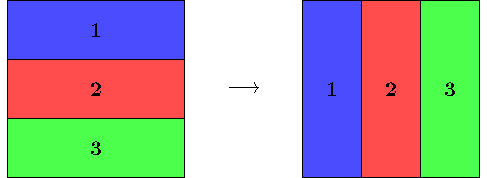
\includegraphics[width=\textwidth]{Simple2D/Start}
\end{frame}

\begin{frame}{Parallelisation Strategy - 3D example}
 \begin{minipage}[b]{.4\textwidth}
 Decomposition in\\ Layout A:
 
  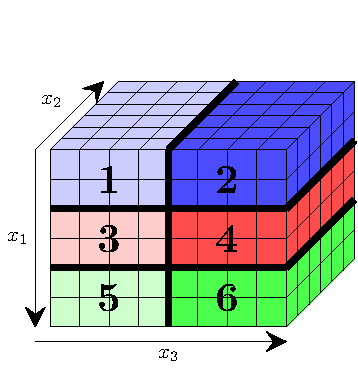
\includegraphics[width=\textwidth]{Parallel3d/End}
 \end{minipage}
 \hspace{.05\textwidth}
 \begin{minipage}[b]{.48\textwidth}
  Decomposition in\\ Layout B:
 
  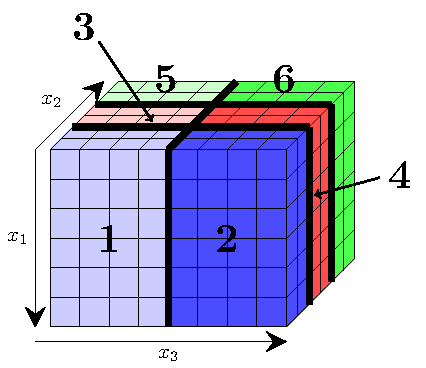
\includegraphics[width=\textwidth]{Parallel3d/End2}
 \end{minipage}
 
 (1,3,5) independent of (2,4,6)
\end{frame}

\begin{frame}{Parallelisation Strategy - 3D example}
\begin{minipage}{.45\textwidth}
 Decomposition in\\ Layout C:\\
 \vspace{1em}
 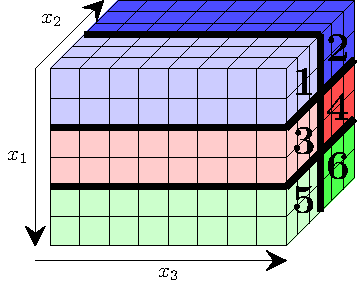
\includegraphics[width=\textwidth]{Parallel3d/Start}
\end{minipage}
\begin{minipage}{.45\textwidth}
 Decomposition in\\ Layout A:
 
 \vspace{-.7em}
 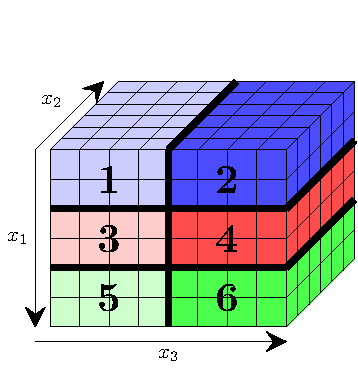
\includegraphics[width=\textwidth]{Parallel3d/End}
\end{minipage}
 
 (1,2) independent of (3,4) and (5,6)
\end{frame}

\begin{frame}{Parallelisation Strategy}
\begin{minipage}{.4\textwidth}
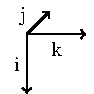
\includegraphics[width=.4\textwidth]{SplitConcat3D/Axes}

  \begin{itemize}
   \item Layout in memory
   \item Numbers indicate contiguous locations in memory
   \item A correct layout change preserves ordering
   \item C-ordering $A[i,j,k]$
  \end{itemize}
  
 \end{minipage}
 \begin{minipage}{.55\textwidth}
 \centering
  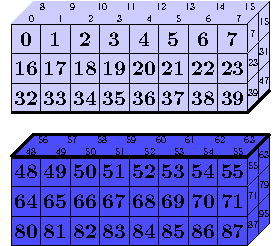
\includegraphics[width=.7\textwidth]{SplitConcat3D/Layout1Distrib1_2}
  \vspace{1em}
  
  \hfill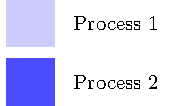
\includegraphics[width=.3\textwidth]{SplitConcat3D/Legend}
  \end{minipage}
\end{frame}

\begin{frame}{Parallelisation Strategy}
 \begin{minipage}{.3\textwidth}
 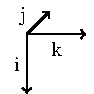
\includegraphics[width=.4\textwidth]{SplitConcat3D/Axes}
 \vspace{4em}
 
  \begin{enumerate}
   \item Split blocks
  \end{enumerate}
  
  \vspace{4em}
 \end{minipage}
 \begin{minipage}{.65\textwidth}
  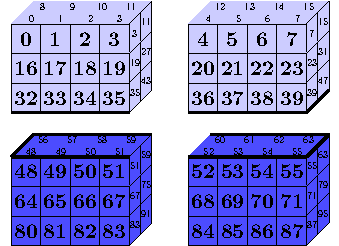
\includegraphics[width=.8\textwidth]{SplitConcat3D/SendBlocksDistrib1_2}
  
  \vspace{1em}
  
  \hfill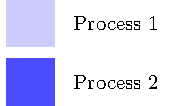
\includegraphics[width=.3\textwidth]{SplitConcat3D/Legend}
 \end{minipage}
\end{frame}

\begin{frame}{Parallelisation Strategy}
 \begin{minipage}{.3\textwidth}
 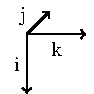
\includegraphics[width=.4\textwidth]{SplitConcat3D/Axes}
 \vspace{4em}
 
  \begin{enumerate}
   \item Split blocks 
   \item Call Alltoall
  \end{enumerate}
  
  \vspace{4em}
 \end{minipage}
 \begin{minipage}{.65\textwidth}
  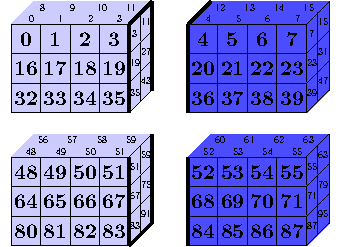
\includegraphics[width=.8\textwidth]{SplitConcat3D/RecvDistrib1_2}
  
  \vspace{1em}
  
  \hfill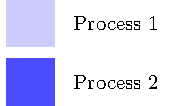
\includegraphics[width=.3\textwidth]{SplitConcat3D/Legend}
 \end{minipage}
\end{frame}

\begin{frame}{Parallelisation Strategy}
 \begin{minipage}{.3\textwidth}
 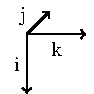
\includegraphics[width=.4\textwidth]{SplitConcat3D/Axes}
 \vspace{4em}
 
  \begin{enumerate}
   \item Split blocks 
   \item Call Alltoall
   \item Transpose to desired shape
  \end{enumerate}
  
  \vspace{4em}
 \end{minipage}
 \begin{minipage}{.65\textwidth}
  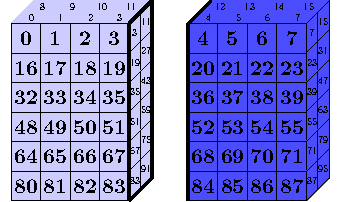
\includegraphics[width=\textwidth]{SplitConcat3D/RecvLayout_2}
  
  \vspace{1em}
  
  \hfill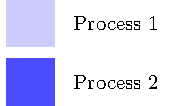
\includegraphics[width=.3\textwidth]{SplitConcat3D/Legend}
 \end{minipage}
\end{frame}

\begin{frame}{Parallelisation Strategy}
 \begin{minipage}{.3\textwidth}
 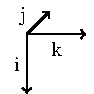
\includegraphics[width=.4\textwidth]{SplitConcat3D/Axes}
 \vspace{4em}
 
  \begin{enumerate}
   \item Split blocks 
   \item Call Alltoall
   \item Transpose to desired shape
  \end{enumerate}
  
  \vspace{4em}
 \end{minipage}
 \begin{minipage}{.65\textwidth}
  \hspace{1pt}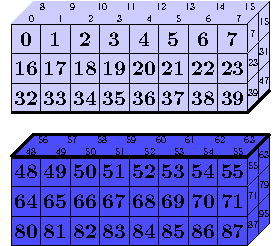
\includegraphics[width=.99\textwidth]{SplitConcat3D/Layout1Distrib1_2}
  
  \vspace{1em}
  
  \hfill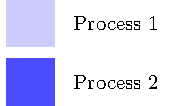
\includegraphics[width=.3\textwidth]{SplitConcat3D/Legend}
 \end{minipage}
\end{frame}

\begin{frame}{Parallelisation Strategy}
 \begin{minipage}{.3\textwidth}
 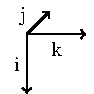
\includegraphics[width=.4\textwidth]{SplitConcat3D/Axes}
 \vspace{4em}
 
  \begin{enumerate}
   \item Split blocks 
   \item Call Alltoall
   \item Transpose to desired shape
  \end{enumerate}
  
  \vspace{4em}
 \end{minipage}
 \begin{minipage}{.65\textwidth}
  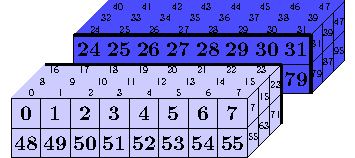
\includegraphics[width=\textwidth]{SplitConcat3D/Layout1Distrib2}\vspace{0pt}
  
  \vspace{1em}
  
  \hfill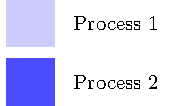
\includegraphics[width=.3\textwidth]{SplitConcat3D/Legend}
 \end{minipage}
\end{frame}

\begin{frame}{Parallelisation Strategy}
 \begin{minipage}{.3\textwidth}
 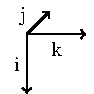
\includegraphics[width=.4\textwidth]{SplitConcat3D/Axes}
 \vspace{4em}
 
  \begin{enumerate}
   \item Split blocks 
   \item Call Alltoall
   \item Transpose to desired shape
  \end{enumerate}
  
  \vspace{4em}
 \end{minipage}
 \begin{minipage}{.65\textwidth}
  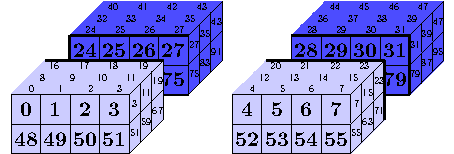
\includegraphics[width=\textwidth]{SplitConcat3D/SendBlocksColouredDistrib2}
  
  \vspace{1em}
  
  \hfill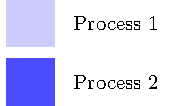
\includegraphics[width=.3\textwidth]{SplitConcat3D/Legend}
 \end{minipage}
\end{frame}

\begin{frame}{Parallelisation Strategy}
 \begin{minipage}{.3\textwidth}
 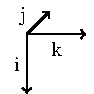
\includegraphics[width=.4\textwidth]{SplitConcat3D/Axes}
 \vspace{4em}
 
  \begin{enumerate}
   \item Split blocks 
   \item Call Alltoall
   \item Transpose to desired shape
  \end{enumerate}
  
  \vspace{4em}
 \end{minipage}
 \begin{minipage}{.65\textwidth}
  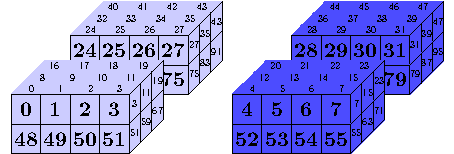
\includegraphics[width=\textwidth]{SplitConcat3D/WrongRecv_2}
  
  \vspace{1em}
  
  \hfill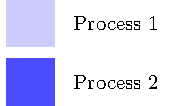
\includegraphics[width=.3\textwidth]{SplitConcat3D/Legend}
 \end{minipage}
\end{frame}

\begin{frame}{Parallelisation Strategy}
 \begin{minipage}{.3\textwidth}
 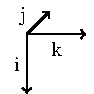
\includegraphics[width=.4\textwidth]{SplitConcat3D/Axes}
 \vspace{4em}
 
  \begin{enumerate}
   \item Split blocks 
   \item Call Alltoall
   \item Transpose to desired shape
  \end{enumerate}
  
  \vspace{4em}
 \end{minipage}
 \begin{minipage}{.65\textwidth}
  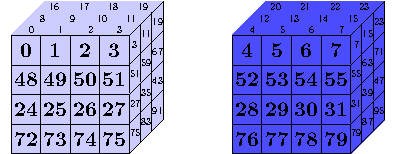
\includegraphics[width=\textwidth]{SplitConcat3D/WrongBlock}
  
  \vspace{1em}
  
  \hfill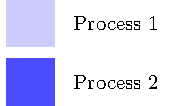
\includegraphics[width=.3\textwidth]{SplitConcat3D/Legend}
 \end{minipage}
\end{frame}

\begin{frame}{Parallelisation Strategy}
 \begin{minipage}{.3\textwidth}
 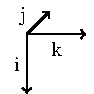
\includegraphics[width=.4\textwidth]{SplitConcat3D/Axes}
 \vspace{4em}
 
  \begin{enumerate}
   \item Split blocks 
   \item Call Alltoall
   \item Transpose to desired shape
  \end{enumerate}
  
  \vspace{4em}
 \end{minipage}
 \begin{minipage}{.65\textwidth}
  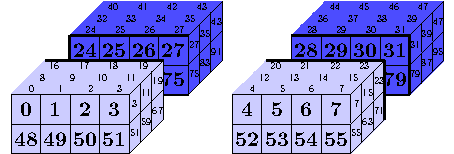
\includegraphics[width=\textwidth]{SplitConcat3D/SendBlocksColouredDistrib2}
  
  \vspace{1em}
  
  \hfill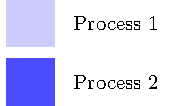
\includegraphics[width=.3\textwidth]{SplitConcat3D/Legend}
 \end{minipage}
\end{frame}

\begin{frame}{Parallelisation Strategy}
 \begin{minipage}{.3\textwidth}
 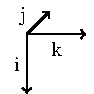
\includegraphics[width=.4\textwidth]{SplitConcat3D/Axes}
 \vspace{1em}
 
  \begin{enumerate}
   \item Split blocks 
   \item Transpose blocks so concatenate direction is first axis
   \item Call Alltoall
   \item Transpose to desired shape
  \end{enumerate}
  
  \vspace{1em}
 \end{minipage}
 \begin{minipage}{.65\textwidth}
  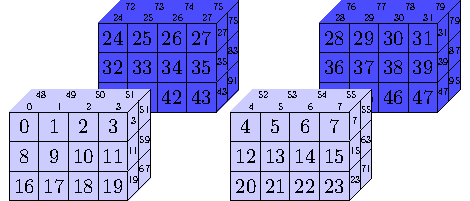
\includegraphics[width=\textwidth]{SplitConcat3D/TransposedSendBlocks}
  
  \vspace{1em}
  
  \hfill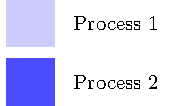
\includegraphics[width=.3\textwidth]{SplitConcat3D/Legend}
 \end{minipage}
\end{frame}

\begin{frame}{Parallelisation Strategy}
 \begin{minipage}{.3\textwidth}
 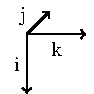
\includegraphics[width=.4\textwidth]{SplitConcat3D/Axes}
 \vspace{1em}
 
  \begin{enumerate}
   \item Split blocks 
   \item Transpose blocks so concatenate direction is first axis
   \item Call Alltoall
   \item Transpose to desired shape
  \end{enumerate}
  
  \vspace{1em}
 \end{minipage}
 \begin{minipage}{.65\textwidth}
  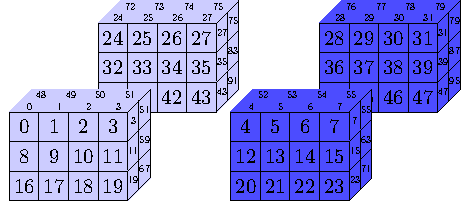
\includegraphics[width=\textwidth]{SplitConcat3D/RightRecv}
  
  \vspace{1em}
  
  \hfill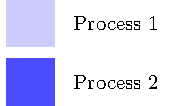
\includegraphics[width=.3\textwidth]{SplitConcat3D/Legend}
 \end{minipage}
\end{frame}

\begin{frame}{Parallelisation Strategy}
 \begin{minipage}{.3\textwidth}
 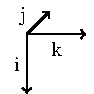
\includegraphics[width=.4\textwidth]{SplitConcat3D/Axes}
 \vspace{1em}
 
  \begin{enumerate}
   \item Split blocks 
   \item Transpose blocks so concatenate direction is first axis
   \item Call Alltoall
   \item Transpose to desired shape
  \end{enumerate}
  
  \vspace{1em}
 \end{minipage}
 \begin{minipage}{.65\textwidth}
  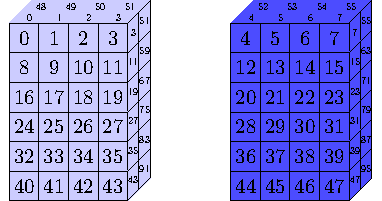
\includegraphics[width=\textwidth]{SplitConcat3D/RecvDistrib2}
  
  \vspace{1em}
  
  \hfill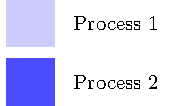
\includegraphics[width=.3\textwidth]{SplitConcat3D/Legend}
 \end{minipage}
\end{frame}

\section{Acceleration with Pyccel}

\begin{frame}{Profiling before Pyccel}
\footnotesize
 \begin{table}[ht]
 \begin{tabular}{|m{.37\textwidth}|c|c|c|c|}
  \hline
          & Total time & Number & Time & Total \\
  Function & excluding sub & of & per call & time \\
          & functions [s] & calls & [s] & [s] \\
  \hline
  \hline
  method 'Alltoall' from mpi4py & 28.193 & 250 & 0.113 & 28.193 \\
  \hline
  numpy.core.multiarray.array & 16.070 & 5689347 & 0.000 & 16.070 \\
  \hline
  bisplev from scipy & 10.009 & 1006666 & 0.000 & 37.819\\
  \hline
  method scipy.interpolate. \_fitpack.\_bispev & 8.503 & 1006666 & 0.000 & 8.503\\
  \hline
  atleast\_1d from numpy & 7.990 & 2915166 & 0.000 & 23.820\\
  \hline
  splev & 7.334 & 901833 & 0.000 & 18.883\\
  \hline
  reshape from numpy & 6.590 & 3397927 & 0.000 & 6.590\\
  \hline
 \end{tabular}
\caption{\label{tab::pure python profile} The results of profiling the pure python implementation}
\end{table}
\end{frame}

\begin{frame}{Profiling after Pyccel}
\footnotesize
 \begin{table}[ht]
\centering
 \begin{tabular}{|m{.37\textwidth}|c|c|c|c|}
  \hline
          & Total time & Number & Time & Total \\
  Function & excluding sub & of & per call & time \\
          & functions [s] & calls & [s] & [s] \\
  \hline
  \hline
  method 'Alltoall' from mpi4py & 2.735 & 250 & 0.011 & 2.735 \\
  \hline
  step in FluxSurfaceAdvection & 1.826 & 5000 & 0.000 & 3.355 \\
  \hline
  parallel\_gradient in ParallelGradient & 1.492 & 1000 & 0.001 & 1.903\\
  \hline
  step in PoloidalAdvection object & 1.420 & 3333 & 0.000 & 3.004\\
  \hline
  method 'solve' from scipy 'SuperLU' & 1.294 & 96666 & 0.000 & 1.294\\
  \hline
  getPerturbedRho in ParallelGradient & 1.022 & 101 & 0.010 & 2.307\\
  \hline
  \_solve\_system\_nonperiodic in SplineInterpolator1D & 0.977 & 123700 & 0.000 & 0.977\\
  \hline
 \end{tabular}
 \caption{\label{tab::final profile} The results of profiling the implementation after pyccelisation}
\end{table}
\end{frame}


\section{Results}

\begin{frame}{Ion Temperature Gradient Test}
 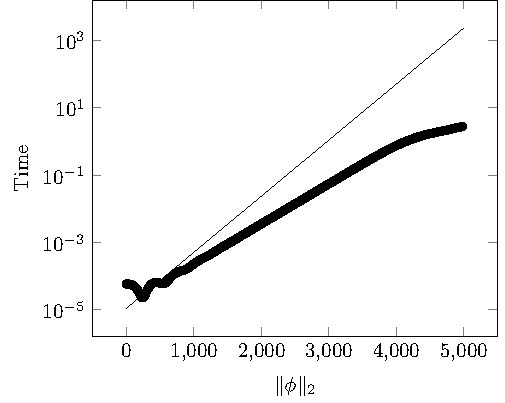
\includegraphics[width=.8\textwidth]{ITG/ITG}
\end{frame}


\begin{frame}{Performance Results}
\centering
 \documentclass{standalone}
\usepackage[dvipsnames]{xcolor}
\usepackage{tikz}
\usepackage{pgfplots}
\usepackage{pgfplotstable}
\pgfplotsset{compat=1.5}
\usetikzlibrary{patterns,decorations.markings}

\definecolor{mygreen}{RGB}{0, 153, 0}

\begin{document}
{
\begin{tikzpicture}
\begin{loglogaxis}[
xlabel={Number of Nodes},
ylabel={Duration of one time step [s]},
legend entries={Pure Fortran,Gfortran,Intel,Manually improved},
legend pos=north east,
xtick={1,2,4,8,16,32},
xticklabels={1,2,4,8,16,32},
minor xtick={3,5,6,7,9,10,11,12,13,14,15,17,18,19,20,21,22,23,24,25,26,27,28,29,30,31},
]
% \addplot[color=black]
%      coordinates{
%      (1 ,  4.8764073060e+02)
%      (2 ,  243.8203653)
%      (4 ,  121.91018265)
%      (8 ,  60.955091325)
%      (16, 30.4775456625)
%      (32, 15.23877283125)
%      };
% \addplot[color=red]
%      coordinates{
%      (1 ,  342.4934561)
%      (2 ,  171.24672805)
%      (4 ,  85.623364025)
%      (8 ,  42.8116820125)
%      (16, 21.40584100625)
%      (32, 10.702920503125)
%      };
% \addplot[color=mygreen]
%      coordinates{
%      (1 ,  122.7)
%      (2 ,  61.35)
%      (4 ,  30.675)
%      (8 ,  15.3375)
%      };
\addplot[
scatter,
only marks,
point meta=explicit symbolic,
scatter/classes={
0={mark=*,mygreen,scale=2},
1={mark=triangle*,red,{scale=2}},
2={mark=triangle*,black,scale=2},
3={mark=square*,red,scale=2}
},
] table[x={nnodes},y={perloop},meta={type}] {Results_withOptimised.dat};
\end{loglogaxis}
\end{tikzpicture}
}
\end{document}
\end{frame}

\begin{frame}{Scaling}
\centering
\hspace{-.08\textwidth}
\begin{minipage}{.45\textwidth}
 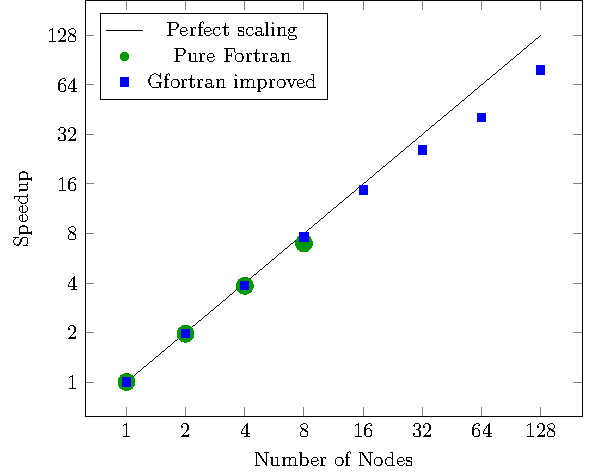
\includegraphics[width=1.1\textwidth]{Scaling/Speedup.pdf}
\end{minipage}
\hspace{.1\textwidth}
\begin{minipage}{.45\textwidth}
 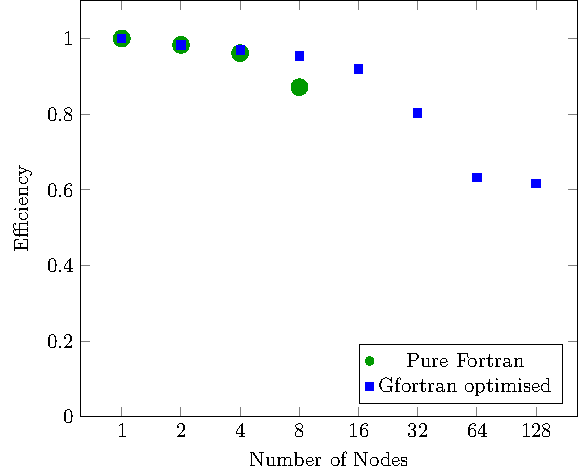
\includegraphics[width=1.1\textwidth]{Scaling/Efficiency.pdf}
\end{minipage}
\end{frame}

\begin{frame}{Conclusion}
\begin{overlayarea}{\textwidth}{5cm}
{\bf Summary:}
 \begin{itemize}
  \item Screw-Pinch Simulation can be effectively written with python
  \item Parallel method has very good scalability
  \item Code translated with pyccel has shorter development time and comparable run-time compared to fortran code
 \end{itemize}
 \vspace{1em}
 
 \only<2->{
 {\bf Future Work:} 
 \begin{itemize}
  \item Extend model to include centre
  \item Tokamak geometry
 \end{itemize}
 \vspace{1em}}

 \only<3->{
 \centering
 Thank you for listening. Any questions?}
\end{overlayarea}
\end{frame}


\end{document}
